\documentclass{article}
\usepackage{amsmath,amsfonts,amsthm,amssymb}
\usepackage{setspace}
\usepackage{fancyhdr}
\usepackage{lastpage}
\usepackage{extramarks}
\usepackage{chngpage}
\usepackage{soul,color}
\usepackage{graphicx,float,wrapfig}
\usepackage{CJK}
\usepackage{algorithm}  
\usepackage{algpseudocode} 
\usepackage{enumerate}
\usepackage{longtable}
\usepackage{listings}
\usepackage{color}
\usepackage{extarrows}
\usepackage{subfigure}
\newcommand{\Class}{Deep Learning}
\newcommand{\ClassInstructor}{Yi Wu}

% Homework Specific Information. Change it to your own
\newcommand{\Title}{Homework 1}
\newcommand{\DueDate}{Mar 10, 2021}
\newcommand{\StudentName}{Runlong Zhou}
\newcommand{\StudentClass}{YaoClass 82}
\newcommand{\StudentNumber}{2018011309}

% In case you need to adjust margins:
\topmargin=-0.45in      %
\evensidemargin=0in     %
\oddsidemargin=0in      %
\textwidth=6.5in        %
\textheight=9.0in       %
\headsep=0.25in         %

% Setup the header and footer
\pagestyle{fancy}                                                       %
\lhead{\StudentName}                                                 %
\chead{\Title}  %
\rhead{\firstxmark}                                                     %
\lfoot{\lastxmark}                                                      %
\cfoot{}                                                                %
\rfoot{Page\ \thepage\ of\ \protect\pageref{LastPage}}                          %
\renewcommand\headrulewidth{0.4pt}                                      %
\renewcommand\footrulewidth{0.4pt}                                      %

%%%%%%%%%%%%%%%%%%%%%%%%%%%%%%%%%%%%%%%%%%%%%%%%%%%%%%%%%%%%%
% Some tools
\newcommand{\enterProblemHeader}[1]{\nobreak\extramarks{#1}{#1 continued on next page\ldots}\nobreak%
                                    \nobreak\extramarks{#1 (continued)}{#1 continued on next page\ldots}\nobreak}%
\newcommand{\exitProblemHeader}[1]{\nobreak\extramarks{#1 (continued)}{#1 continued on next page\ldots}\nobreak%
                                   \nobreak\extramarks{#1}{}\nobreak}%

\newcommand{\homeworkProblemName}{}%
\newcounter{homeworkProblemCounter}%
\newenvironment{homeworkProblem}[1][Problem \arabic{homeworkProblemCounter}]%
  {\stepcounter{homeworkProblemCounter}%
   \renewcommand{\homeworkProblemName}{#1}%
   \section*{\homeworkProblemName}%
   \enterProblemHeader{\homeworkProblemName}}%
  {\exitProblemHeader{\homeworkProblemName}}%

\newcommand{\homeworkSectionName}{}%
\newlength{\homeworkSectionLabelLength}{}%
\newenvironment{homeworkSection}[1]%
  {% We put this space here to make sure we're not connected to the above.

   \renewcommand{\homeworkSectionName}{#1}%
   \settowidth{\homeworkSectionLabelLength}{\homeworkSectionName}%
   \addtolength{\homeworkSectionLabelLength}{0.25in}%
   \changetext{}{-\homeworkSectionLabelLength}{}{}{}%
   \subsection*{\homeworkSectionName}%
   \enterProblemHeader{\homeworkProblemName\ [\homeworkSectionName]}}%
  {\enterProblemHeader{\homeworkProblemName}%

   % We put the blank space above in order to make sure this margin
   % change doesn't happen too soon.
   \changetext{}{+\homeworkSectionLabelLength}{}{}{}}%

\newcommand{\Answer}{\textbf{Answer:} }
\newcommand{\Acknowledgement}[1]{\ \\{\bf Acknowledgement:} #1}

%%%%%%%%%%%%%%%%%%%%%%%%%%%%%%%%%%%%%%%%%%%%%%%%%%%%%%%%%%%%%


%%%%%%%%%%%%%%%%%%%%%%%%%%%%%%%%%%%%%%%%%%%%%%%%%%%%%%%%%%%%%
% Make title
\title{\textmd{\bf \Class: \Title}\\{\large Instructed by \textit{\ClassInstructor}}\\\normalsize\vspace{0.1in}\small{Due\ on\ \DueDate}}
\date{}
\author{\textbf{\StudentName}\ \ \StudentClass\ \ \StudentNumber}
%%%%%%%%%%%%%%%%%%%%%%%%%%%%%%%%%%%%%%%%%%%%%%%%%%%%%%%%%%%%%


%%%%%%%%%%%%%%%%%%%%%%%%%%%%%%%%%%%%%%%%%%%%%%%%%%%%%%%%%%%%%
% Listing Settings
\definecolor{mygreen}{rgb}{0,0.6,0}
\definecolor{mygray}{rgb}{0.5,0.5,0.5}
\definecolor{mymauve}{rgb}{0.58,0,0.82}

\lstset{
  aboveskip=1em,                   % above skip space
  backgroundcolor=\color[rgb]{0.9,0.9,0.9},
                                   % choose the background color; you must add \usepackage{color} or \usepackage{xcolor}; should come as last argument
  basicstyle=\ttfamily,            % the size of the fonts that are used for the code
  breakatwhitespace=false,         % sets if automatic breaks should only happen at whitespace
  breaklines=true,                 % sets automatic line breaking
  captionpos=b,                    % sets the caption-position to bottom
  commentstyle=\color{mygreen},    % comment style
  deletekeywords={...},            % if you want to delete keywords from the given language
  escapeinside={\%*}{*)},          % if you want to add LaTeX within your code
  extendedchars=true,              % lets you use non-ASCII characters; for 8-bits encodings only, does not work with UTF-8
  frame=single,	                   % adds a frame around the code
  keepspaces=true,                 % keeps spaces in text, useful for keeping indentation of code (possibly needs columns=flexible)
  keywordstyle=\color{blue},       % keyword style
  morekeywords={algexpr, frac, sqrt, pwr, b1, b2, b3, ln, sin, term},  
                                   % if you want to add more keywords to the set
  numbers=left,                    % where to put the line-numbers; possible values are (none, left, right)
  numbersep=5pt,                   % how far the line-numbers are from the code
  numberstyle=\color{mygray},      % the style that is used for the line-numbers
  rulecolor=\color{black},         % if not set, the frame-color may be changed on line-breaks within not-black text (e.g. comments (green here))
  showspaces=false,                % show spaces everywhere adding particular underscores; it overrides 'showstringspaces'
  showstringspaces=false,          % underline spaces within strings only
  showtabs=false,                  % show tabs within strings adding particular underscores
  stepnumber=2,                    % the step between two line-numbers. If it's 1, each line will be numbered
  stringstyle=\color{mymauve},     % string literal style
  tabsize=2,	                   % sets default tabsize to 2 spaces
  title=\lstname,                  % show the filename of files included with \lstinputlisting; also try caption instead of title
  xleftmargin=2em,                 % left margin
  xrightmargin=2em,                % right margin
}
%%%%%%%%%%%%%%%%%%%%%%%%%%%%%%%%%%%%%%%%%%%%%%%%%%%%%%%%%%%%%


\renewcommand{\algorithmicrequire}{\textbf{Input:}}  % Use Input in the format of Algorithm  
\renewcommand{\algorithmicensure}{\textbf{Output:}} % Use Output in the format of Algorithm  


\newcommand*{\dif}{\mathop{}\!\mathrm{d}}
\newcommand*{\img}{\mathrm{i}}
\newcommand*{\e}{\mathrm{e}}
\newcommand*{\dps}{\displaystyle}
\newcommand*{\lf}{\left\lfloor}
\newcommand*{\rf}{\right\rfloor}
\newcommand*{\lc}{\left\lceil}
\newcommand*{\rc}{\right\rceil}
\newcommand*{\ovt}[2]{\dps{\mathop{#1}^{#2}}}

\newtheorem{lma}{Lemma}

\newcommand{\lm}[1]{\textbf{Lemma \ref{#1}}}
\newcommand{\lgd}[2]{\left(\frac{#1}{#2}\right)}
\newcommand{\ds}[2]{\dps \frac{\partial #1}{\partial #2}}
\newcommand{\bds}[2]{\dps \frac{\partial}{\partial #2}\left(#1\right)}
\newcommand{\Eds}[2]{\dps \frac{\partial^2 #1}{\partial #2^2}}
\newcommand{\eds}[3]{\dps \frac{\partial^2 #1}{\partial #2\partial #3}}
\newcommand{\E}[1]{\mathbb{E}\left[#1\right]}
\newcommand{\Var}[1]{\mathrm{Var}\left[#1\right]}
\newcommand{\Cov}[1]{\mathrm{Cov}\left[#1\right]}

\newcommand{\Fig}[1]{\textbf{Figure\ \ref{#1}}}

\begin{document}
\begin{spacing}{1.1}
\maketitle \thispagestyle{empty}
%\cite{}
%%%%%%%%%%%%%%%%%%%%%%%%%%%%%%%%%%%%%%%%%%%%%%%%%%%%%%%%%%%%%
% Begin edit from here

\begin{homeworkProblem}[1.1]

\Answer 
\begin{itemize}

\item \textbf{Convolutional layer.}
\[\frac{\dif (\text{weight}(j,k)\star z(k))(h,w)}{\dif z(a,b,c)}=\mathbb{I}\{k=a,\ h\le b<h+k_H,\ w\le c<w+k_W\}\text{weight}(j,k,b-h,c-w),\]
hence,
\[\begin{split}
    \frac{\dif y(j,h,w)}{\dif z(a,b,c)}&=\sum_{k=0}^{C_{\text{in}}-1}\mathbb{I}\{k=a,\ h\le b<h+k_H,\ w\le c<w+k_W\}\text{weight}(j,k,b-h,c-w)\\
    &=\mathbb{I}\{h\le b<h+k_H,\ w\le c<w+k_W\}\text{weight}(j,a,b-h,c-w).
\end{split}\]
Further,
\[\begin{split}
    \frac{\dif L}{\dif z(a, b, c)}&=\sum_{j,h,w}\frac{\dif L}{\dif y(j,h,w)}\cdot \frac{\dif y(j,h,w)}{\dif z(a, b, c)}\\
    &=\sum_{j=0}^{C_{\text{out}}-1}\sum_{h=b-k_H+1}^b\sum_{w=c-k_W+1}^c \text{weight}(j,a,b-h,c-w)\frac{\dif L}{\dif y(j,h,w)}.
\end{split}\]

\[\frac{\dif y(j,h,w)}{\dif \text{weight}(j,a,b,c)}=z(a,h+b,w+c),\]
hence,
\[\frac{\dif L}{\dif \text{weight}(j,a,b,c)}=\sum_{h,w} z(a,h+b,w+c)\frac{\dif L}{\dif y(j,h,w)}.\]

\[\frac{\dif L}{\dif \text{bias}(j)}=\sum_{h,w} \frac{\dif L}{\dif y(j,h,w)}.\]

\item \textbf{Max-pooling layer.}
\[\frac{\dif y(j,h,w)}{\dif z(a, b, c)}=\mathbb{I}\left\{j=a,\ (b,c)=\arg\max_{(m,n)\le (k_H-1,k_W-1)}z(j,\text{stride}[0]\times h+m,\text{stride}[1]\times w+n)\right\},\]
hence,
\[\begin{split}
    &\quad \frac{\dif L}{\dif z(a, b, c)}\\
    &=\sum_{j,h,w}\frac{\dif L}{\dif y(j,h,w)}\cdot \frac{\dif y(j,h,w)}{\dif z(a, b, c)}\\
    &=\sum_{h,w}\mathbb{I}\left\{(b,c)=\arg\max_{(m,n)\le (k_H-1,k_W-1)}z(a,\text{stride}[0]\times h+m,\text{stride}[1]\times w+n)\right\}\frac{\dif L}{\dif y(a,h,w)}.
\end{split}\]

\item \textbf{Tanh.}
\[\frac{\dif y}{\dif z}=\frac{(\e^z+\e^{-z})^2-(\e^z-\e^{-z})^2}{(\e^z+\e^{-z})^2}=1-y^2,\]
hence,
\[\frac{\dif L}{\dif z}=\frac{\dif L}{\dif y}\cdot \frac{\dif y}{\dif z}=(1-y^2)\frac{\dif L}{\dif y}.\]

\end{itemize}

\end{homeworkProblem}

\begin{homeworkProblem}[2]

\Answer
\begin{enumerate}

\item Three settings with smallest test losses are listed as follows:

\begin{figure}[H] 
\centering 
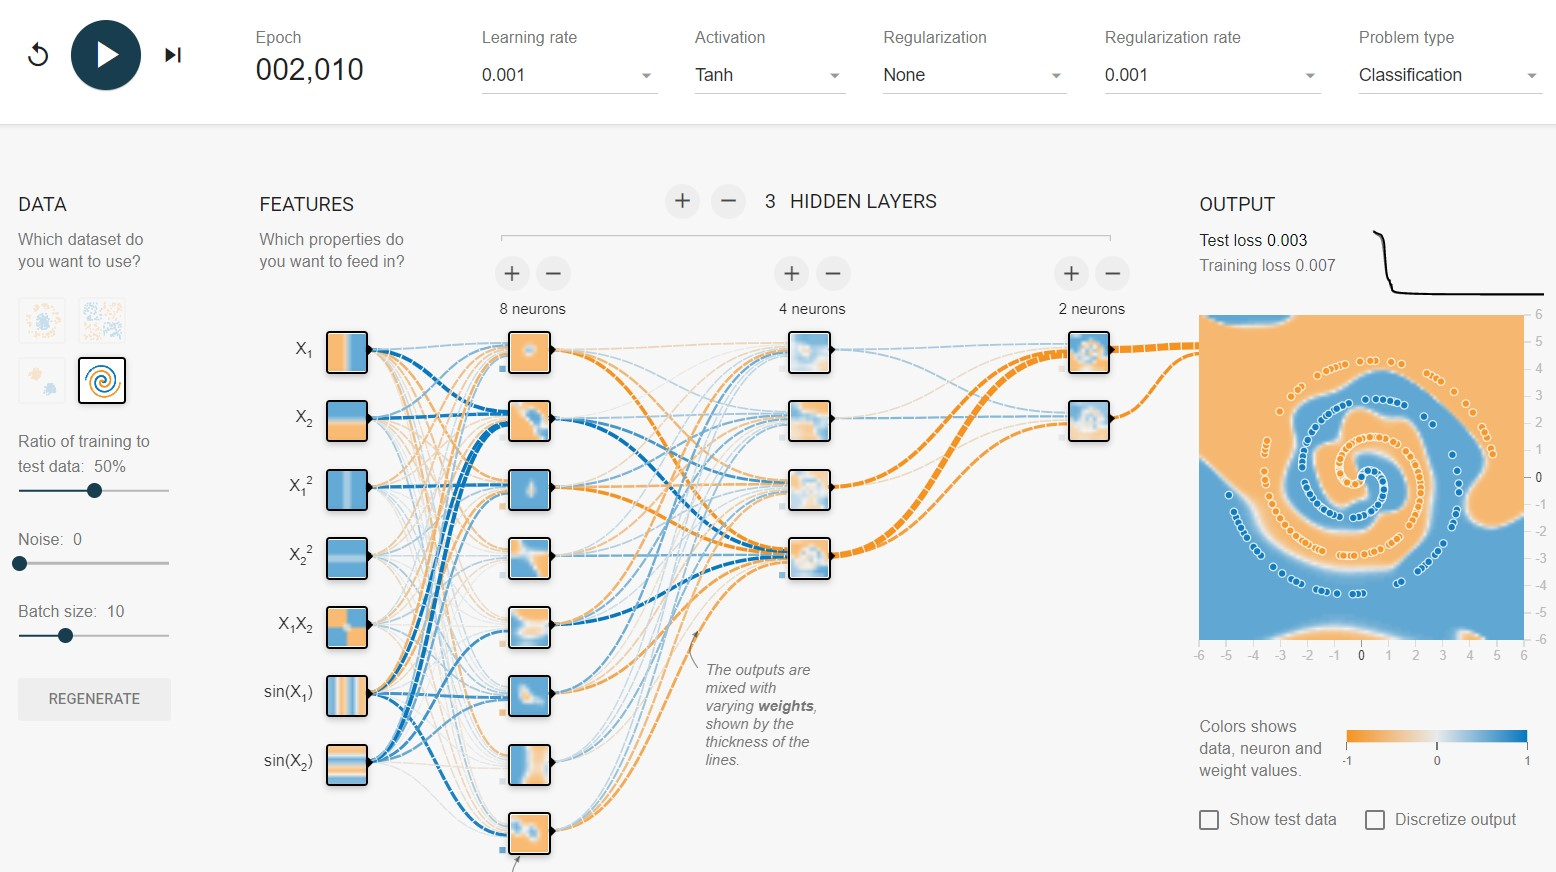
\includegraphics[scale=0.4]{003.jpg}
\caption{Test loss $=0.003$}
\end{figure}

\begin{figure}[H] 
\centering 
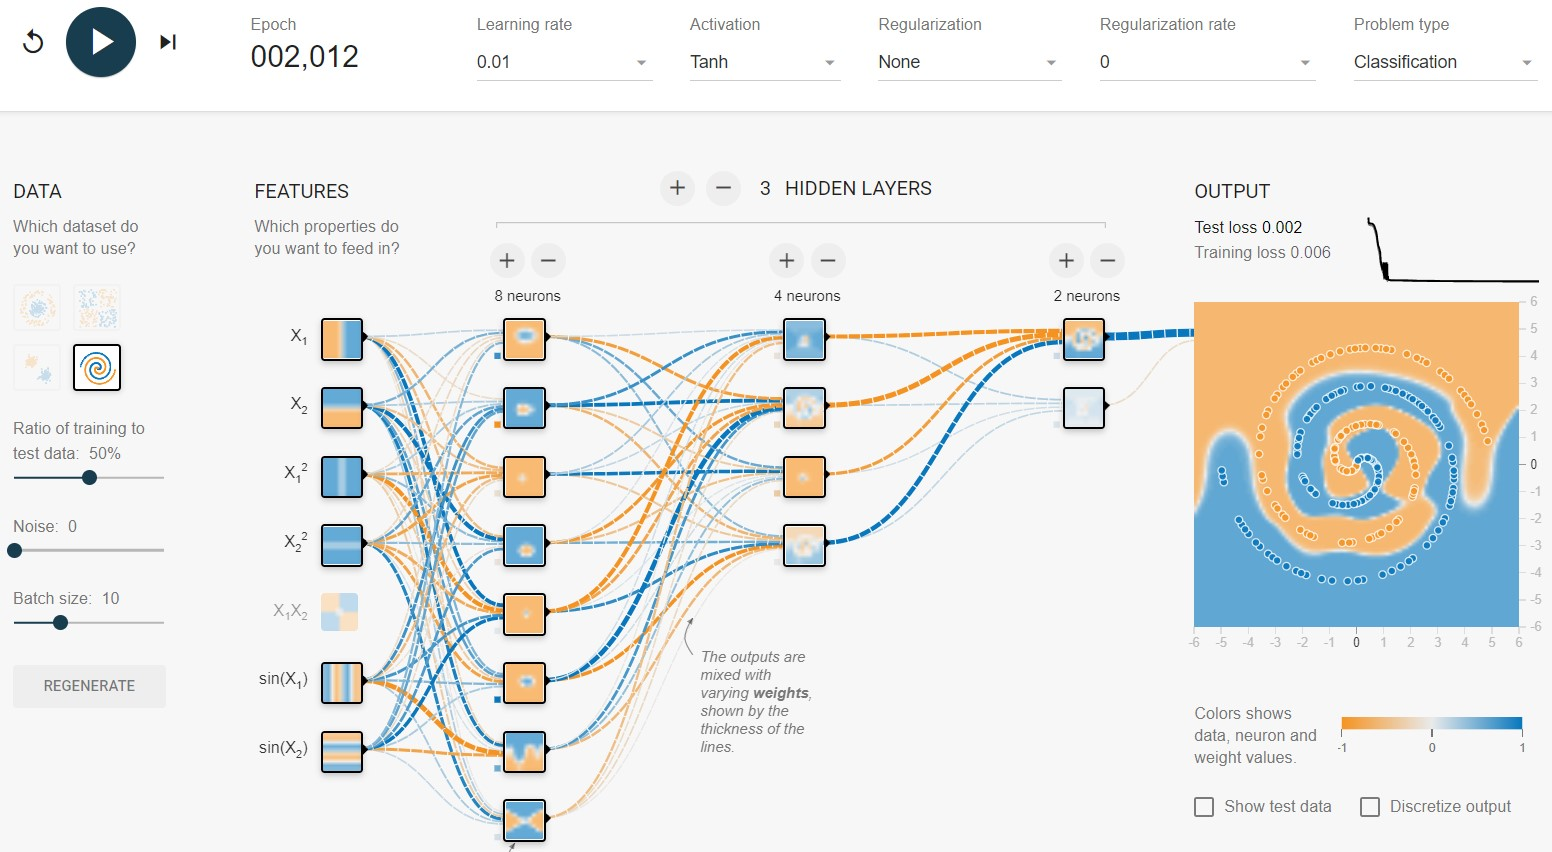
\includegraphics[scale=0.4]{002.jpg}
\caption{Test loss $=0.002$}
\end{figure}

\begin{figure}[H] 
\centering 
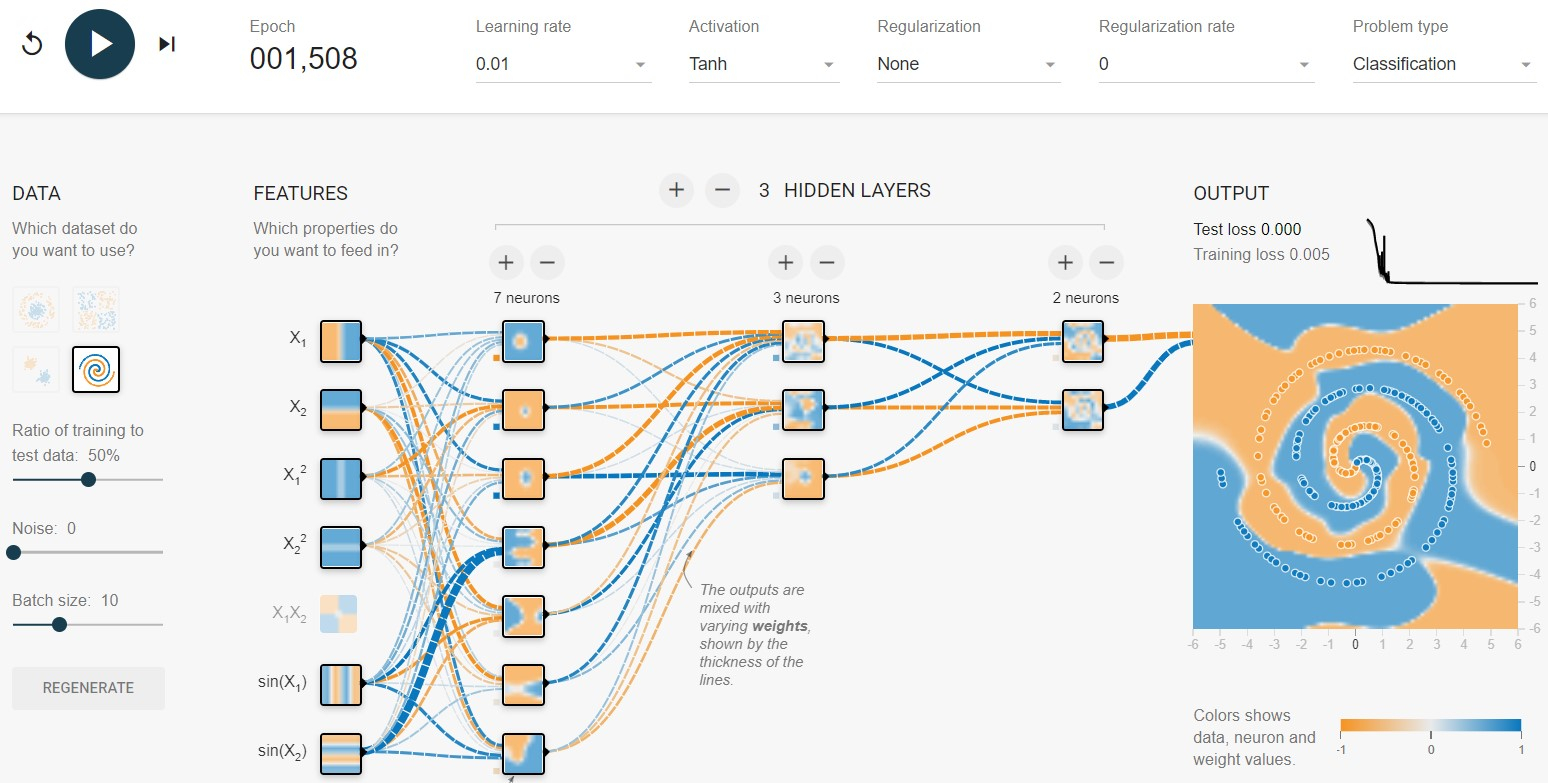
\includegraphics[scale=0.4]{000.jpg}
\caption{Test loss $=0.000$} 
\end{figure}

The first setting includes all the kernels so it works fairly well. By observing that $x_1x_2$ had diminishing weights during training, it was removed in the second setting. By cutting more neurons out, a lighter network (the last setting) is attained.

\item \textbf{Learning rate:} Higher learning rates make losses decrease faster in the beginning, but the losses are more likely to jitter afterwards. Lower learning rates give more smooth optimizing process, but the convergence rate is slower.

\textbf{Hidden nodes:} More hidden nodes make convergence slower and do not necessarily mean lower test loss. Extremely small number of nodes cannot learn well either.

\textbf{Regularization:} Higher regularization factor makes convergence faster, but may converge to a worse model since the some weights are suppressed to lower values, nullifying some nodes.

\end{enumerate}

\end{homeworkProblem}

% End edit to here
%%%%%%%%%%%%%%%%%%%%%%%%%%%%%%%%%%%%%%%%%%%%%%%%%%%%%%%%%%%%%

\end{spacing}
\end{document}

%%%%%%%%%%%%%%%%%%%%%%%%%%%%%%%%%%%%%%%%%%%%%%%%%%%%%%%%%%%%%
